\section{Learning Hamiltonians and resolving resonance}
\label{sec:learning-kam}

\subsection{A real energy with complex trainable representations}
Hamiltonian learning differentiates a scalar energy to obtain the conservative field \citep{Greydanus2019,Chen2022}. Here its target is the 12-configuration, 24-phase-dimensional variable-mass Kirchhoff model with 20 geometric integration cells and an ideal uniform axial magnetic bias, denoted by $H_{\mathrm{ideal}}$. The complete coil plant has a different magnetic potential. Fluid, contact and damping forces are excluded from these conservative labels. Thus learning tests approximation of the declared mechanical energy; its deployment additionally requires the physical port interface.

Use the dimensionless canonical state $z=(Q,P)$ and energy $h=H/E_0$, with $\tau=\omega_0t$. After the physical canonical scaling, define
\begin{equation}
 \begin{aligned}
 \xi&=(Q+iP)/\sqrt2,\\
 \chi&=(Q-iP)/\sqrt2.
 \end{aligned}
 \label{eq:learn-complex-coordinate}
\end{equation}
On the real slice $\chi=\bar\xi$; in a holomorphic extension they are independent. The inverse change of variables gives
\begin{equation}
 \begin{aligned}
 \partial_\chi&=(\partial_Q+i\partial_P)/\sqrt2,\\
 \{\xi_j,\chi_k\}&=-i\delta_{jk},\\
 \xi'&=-ih_\chi+iR/\sqrt2,
 \end{aligned}
 \label{eq:learn-complex-field}
\end{equation}
where $R$ enters the momentum equation. The same derivative convention must enter both the training loss and the predictor. Complex parameters do not make the physical energy complex-valued, and an imaginary energy output alone does not implement physical Rayleigh damping.

For training, $x=Dz$, where $D=\operatorname{diag}(\sqrt\nu,\sqrt\nu)/a$, $\nu=\omega/\omega_0$, and $a=0.08$. This additional scaling is not canonical: $\nabla_zh=D\nabla_xh$ and $x'=DJD\nabla_xh$. All models add a residual $r_\theta$ to the same quadratic prior $h_2=a^2\|x\|^2/2$.

The finite analytic model spans every cubic and quartic mechanical residual with momentum degree zero or two: $Q^3$, $Q^4$, $QP^2$, and $Q^2P^2$, contributing respectively 364, 1365, 936, and 6084 coefficients. These 8749 real parameters describe the stated mechanical class, rather than all quartics in 24 variables. The full complex network has two width-48 complex hidden layers and a complex readout, totaling 3552 complex or 7104 real parameters. It uses both complex inputs and conjugates, split activation $\sigma(u)=\tanh(\operatorname{Re}u)+i\tanh(\operatorname{Im}u)$, a cubic gate, and averaging over $P\mapsto-P$. All real and imaginary weights are trained. The gate preserves the quadratic prior; the averaging preserves momentum parity. Neither ensures convexity in momentum.

The mechanical complex network uses 13440 real parameters and predicts a lower-triangular matrix $L(Q)$ with positive exponential diagonal and $L(0)=I$, together with a potential residual. Its energy is
\begin{equation}
 \begin{aligned}
 h_\theta&=\tfrac12a^2x_P^TLL^Tx_P\\
 &\quad+\tfrac12a^2\|x_Q\|^2+V_\theta(x_Q),\\
 (h_\theta)_{PP}&=D_\nu LL^TD_\nu,
 \end{aligned}
 \label{eq:learn-spd}
\end{equation}
where $D_\nu=\operatorname{diag}\sqrt\nu$. For finite real outputs, $v^T(h_\theta)_{PP}v=\|L^TD_\nu v\|^2>0$ for every $v\ne0$. Hence the fixed-$Q$ momentum-to-velocity map is a linear bijection in exact arithmetic. This establishes structure without a uniform conditioning or physical mass-error bound.

Split activation is real analytic but not holomorphic in one complex argument. A valid extension replaces conjugate inputs by independent variables and uses
\begin{equation}
 \begin{aligned}
 \sigma^{\mathbb C}(u,v)&=\tanh((u+v)/2)\\
 &\quad+i\tanh((u-v)/(2i)),
 \end{aligned}
 \label{eq:learn-analytic-extension}
\end{equation}
with trained coefficients and their conjugates frozen. This gives a local holomorphic extension on domains avoiding all layer poles. No common pole margin or complex-domain approximation norm is certified by the reported training.

\subsection{Frozen training and mechanical diagnostics}
The experiment uses 1024 training and 256 validation states sampled uniformly in $[-1,1]^{24}$ with data seed 51001. Each architecture is trained with seeds 51001--51003, 1200 Adam updates and batch size 128. Learning rates are $10^{-3}$ for the polynomial and $3\times10^{-3}$ for the networks; the gradient clipping threshold is 10. With $r_*=h_{\mathrm{ideal}}-h_2$, the actual objective is
\begin{equation}
 \begin{aligned}
 \mathcal L&=\operatorname{mean}\left[\left(\frac{D(\nabla_xr_\theta-\nabla_xr_*)}{s_g}\right)^2\right]\\
 &\quad+0.15\operatorname{mean}\left[\left(\frac{r_\theta-r_*}{s_h}\right)^2\right],
 \end{aligned}
 \label{eq:learn-objective}
\end{equation}
where $s_h=0.00954395736$ is the training residual-energy standard deviation and $s_g=0.4661470702$ is its canonical-gradient RMS. Validation selects checkpoints every 50 updates, also checking the first update. All nine weights are frozen before generating 512 independent test labels in $[-1,1]^{24}$ and 256 wider-domain labels in $[-1.5,1.5]^{24}$ using seed 510990. Computation uses float64/complex128, one CPU thread and PyTorch 2.5.1; the recorded invocation takes approximately 410.8\,s.

Table~\ref{tab:learn-errors} and Figure~\ref{fig:learning} report the canonical-field relative $L^2$ error, $\|J\nabla(h_\theta-h_*)\|_2/\|J\nabla h_*\|_2$, over each sample set. The unrestricted complex network is most accurate under this budget, whereas the SPD model alone guarantees positive momentum curvature. The quadratic prior gives 63.094\% test error; a smaller historical 48-feature readout gives 62.964\%. Parameter counts, function classes, learning rates and per-update costs differ. These comparisons do not isolate an advantage of complex over real parameterization. In particular, finite-budget Adam does not establish the least-squares optimum of the polynomial class.

\begin{table*}[t]
 \centering
 \caption{Frozen learning results: ranges over three seeds. The last column counts nonpositive momentum Hessians at eight prescribed test states for each seed. Wider-domain samples use a 1.5-fold coordinate box.}
 \label{tab:learn-errors}
 \small\setlength{\tabcolsep}{3.5pt}
 \begin{tabular}{lrrrr}
 \toprule
 Model & Real parameters & Test field error (\%) & Wider-domain error (\%) & Nonpositive $h_{PP}$ \\
 \midrule
 Mechanical polynomial & 8749 & 35.249--35.282 & 59.743--60.273 & 4/4/4 \\
 Full complex hidden layers & 7104 & 3.241--3.700 & 8.410--9.063 & 2/2/4 \\
 SPD mechanical complex & 13440 & 11.415--11.553 & 20.651--21.917 & 0/0/0 \\
 \bottomrule
 \end{tabular}
\end{table*}

At eight test and eight wider-domain states per seed, we separately evaluate Hessians, energy second differences, and the Legendre equation $\partial_Ph_\theta(Q,\widehat P)=\partial_Ph_*(Q,P)$. Initialization at the true $P$ makes this a favorable local test. A small equation residual can coexist with a large recovered-momentum error. Some solver progress flags are false despite residuals near roundoff; the unrestricted complex model also has genuinely non-negligible inversion residuals. Its maximum sampled test Hessian condition number reaches $1.67\times10^5$. The SPD model's sampled wider-domain condition number reaches approximately 1811; positivity does not establish accurate inertia. The maximum sampled test Hessian relative errors are 47.49\%, 5.82\% and 17.05\%, and maximum relative recovered-momentum errors are 27.30, 0.6267 and 0.5044 for polynomial, complex and SPD models, respectively. Independently regenerated labels and directional second differences confirm the saved negative-curvature signs.

For deployment, the desired correction to the learned field is $(-\delta g_P,+\delta g_Q)$, with $\delta g=\nabla h_\theta-\nabla h_*$. Coil currents directly alter only the momentum equation. A separate constrained allocation therefore tests the reachable part of $\delta g_Q$ while retaining the configuration-velocity error and the force component outside the coil image. Across three models, three seeds and eight states, all 72 corrected allocations finish; effective port rank is five at relative cutoff $10^{-8}$, and some currents reach the 2\,A boundary. The after/before total-field-error ratios are 0.8845--0.9898, 0.8959--0.9960 and 0.8482--0.9965 for polynomial, complex and SPD models. This is a static allocation diagnostic with a declared 0.25\,s current-change window. It does not integrate a learned closed loop.


\begin{figure*}[t]
\centering
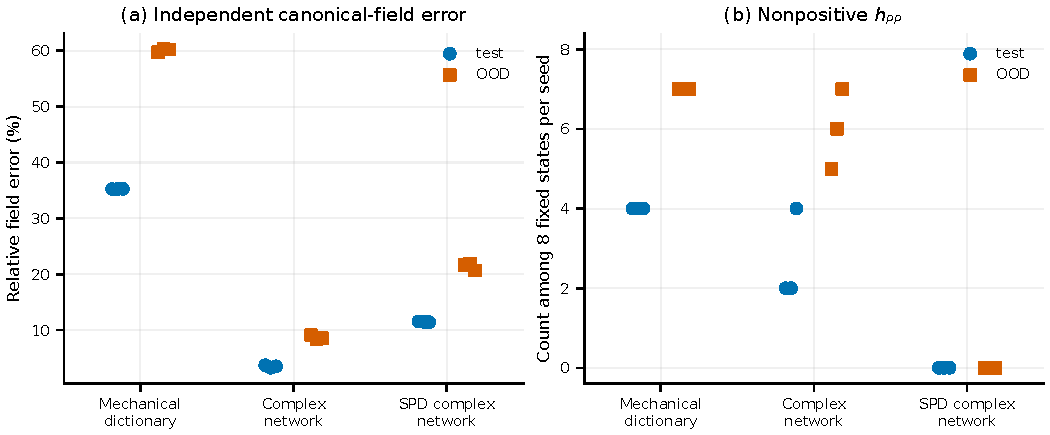
\includegraphics[width=\textwidth]{../figures/learning.pdf}
\caption{Frozen Hamiltonian-learning comparison. Each point denotes one of three training seeds; the left panel gives independent test and wider-domain canonical-field errors. The right panel counts nonpositive momentum Hessians among eight prescribed states per seed in each split. These finite samples are not uniform domain bounds. All models were trained on the ideal-bias Hamiltonian, not the full-coil potential.}
\label{fig:learning}
\end{figure*}

\subsection{From empirical error to a persistence hypothesis}
Two distinct error arguments preserve the learning-to-dynamics connection. For a finite basis, write $h_\theta=h_0+\sum c_{\theta j}\psi_j$ and $h_*=h_0+\sum c_{*j}\psi_j+R$. Stack sampled derivative features into $A$, remove the constant gauge, and use the same observation normalization $N_o$ for all residuals. If $G=A^TA/N_o\succeq\lambda I$, then
\begin{equation}
 \begin{aligned}
 \|h_\theta-h_*\|_{\mathcal X}
 &\le B_{\mathcal X}\frac{r+e}{\sqrt\lambda}+\|R\|_{\mathcal X},\\
 B_{\mathcal X}&=\Big(\sum_j\|\psi_j\|_{\mathcal X}^2\Big)^{1/2}.
 \end{aligned}
 \label{eq:learn-gram-bound}
\end{equation}
Here $r$ is the fitted observation residual and $e$ includes observation error and sampled derivatives of $R$. The proof uses the least singular value and Cauchy--Schwarz; it requires neither independent samples nor optimal fitting. The norm may be real $C^\ell$ or analytic supremum on a specified complex domain. Integral observations require their endpoint and quadrature errors, and exported coefficients require rounding bounds. The old two-mode full-cosine model retained all 35 quartic directions, realized by a cosine coefficient and 34 orthogonal polynomial directions. Its Gram bound does not transfer to the new 8749-feature dictionary.

A second, conditional argument \citep{Chen2022} combines parameter covering, Hoeffding concentration, Poincar\'e and interpolation. Let $\mathcal D=\mathbb T^n\times B$, $d=2n$, $p>d$, $\ell\ge1$, and integer $s>\ell+d/p$. Require independent samples with density at least $m_0$, a bounded realified parameter cube, uniformly bounded gradient residuals and parameter Lipschitz constant, and a uniform gauge-fixed $W^{s,p}$ bound $M_s$. Then, with probability at least $1-\delta$, simultaneously for the class,
\begin{equation}
 \begin{aligned}
 \|e_\theta\|_{C^\ell}&\le E_\theta,\\
 E_\theta&=C_{\mathrm{GN}}(G_\theta+M_s^\alpha G_\theta^{1-\alpha}),\\
 \alpha&=\frac{\ell-1+d/p}{s-1},
 \end{aligned}
 \label{eq:learn-statistical-bound}
\end{equation}
where $G_\theta=C_Pm_0^{-1/p}(\widehat R_\theta+\Gamma)^{1/p}$ and $\Gamma$ is the explicit covering penalty derived in the Supplement. This is a uniform statistical implication, not an Adam convergence theorem. Neither argument has all its constants certified for the present networks. Finite sampled gradient errors alone cannot supply them: already in one scalar variable $w$, the polynomial $c\prod_j(w-w_j)^2$ preserves zero values and first derivatives at the sample points while its complex-domain norm can grow arbitrarily with $c$.

\begin{figure*}[t]
\centering
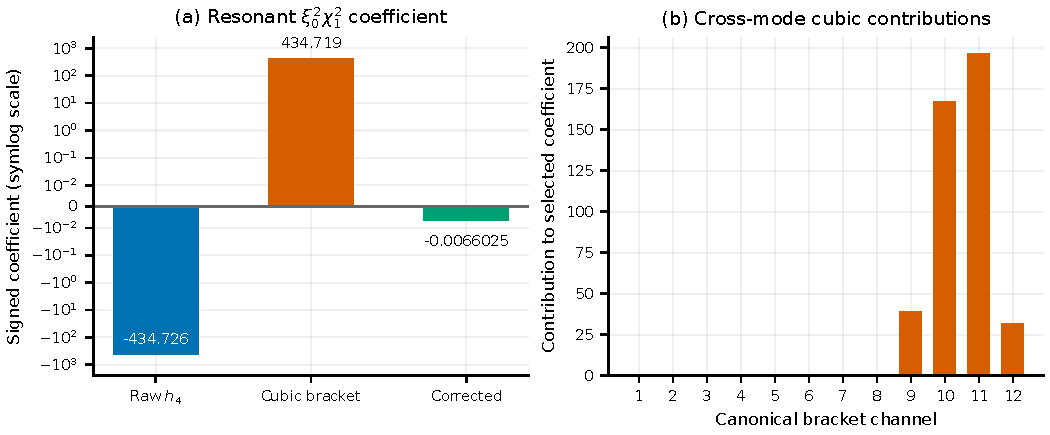
\includegraphics[width=\textwidth]{../figures/resonance.pdf}
\caption{First-pair quartic resonance diagnostic. Left: raw quartic coefficient, all-12-channel cubic-elimination correction and their small residual on a symmetric logarithmic scale. Right: the contributions of four external torsional bracket channels to the cubic-elimination correction, with channel indices numbered from one. All 12 canonical channels are retained in the computation. The original first-pair subspace is not invariant, so this restricted coefficient does not establish full-dimensional KAM nondegeneracy.}
\label{fig:resonance}
\end{figure*}

\subsection{The resonant three-dimensional mechanical model}
The actual linearized ideal-bias model has four $1{:}1$ bending pairs with frequency ratios $1$, $6.21276315$, $17.89814255$ and $80.07400435$. At cutoff $10^{-10}$, enumeration of all 2600 cubic monomials finds no resonances and minimum divisor one; among 17550 quartics, 206 lie in the homological kernel, including 78 action terms and 128 non-action terms. The paired degeneracy follows from circular-rod axial symmetry; the numerical cutoff is only its finite-order diagnostic.

For $h=h_2+h_3+h_4+\cdots$, $h_2=\sum_j\nu_j\xi_j\chi_j$, the homological equation and its cubic solution are
\begin{equation}
 \begin{aligned}
 \{h_2,\xi^\alpha\chi^\beta\}
 &=i\nu\cdot(\alpha-\beta)\xi^\alpha\chi^\beta,\\
 (W_3)_{\alpha\beta}&=\frac{i(h_3)_{\alpha\beta}}{\nu\cdot(\alpha-\beta)}.
 \end{aligned}
 \label{eq:learn-homological}
\end{equation}
Thus $\{h_2,W_3\}=-h_3$, and the Lie expansion gives the resonant quartic
\begin{equation}
 Z_4=\Pi_{\mathrm{res}}\left(h_4+\tfrac12\{h_3,W_3\}\right).
 \label{eq:learn-resonant-quartic}
\end{equation}
For the restriction to the first bending pair, all 12 canonical bracket channels are retained. Differentiating the full gradient twice in the four selected real coordinates supplies every cubic monomial that can survive this restriction after one derivative; terms containing two external variables cannot contribute. Four external torsional channels provide the nonzero correction to the coefficient of $\xi_0^2\chi_1^2$:
\begin{equation}
 \begin{aligned}
 &-434.7256304212535+434.719027922014\\
 &\qquad\simeq-0.006602499239534154.
 \end{aligned}
 \label{eq:learn-cancellation}
\end{equation}
The cancellation exceeds four orders of magnitude (Figure~\ref{fig:resonance}). The accepted calculation uses reverse automatic differentiation, with quartic permutation defect $2.27\times10^{-13}$ and independent scalar-derivative checks. Its raw coefficient differs from radius extrapolation by $7.26\times10^{-7}$. An earlier mixed-mode derivative tensor failed permutation symmetry (defect 1738.9) and is excluded; the failed artifact remains preserved. These checks validate finite-order numerical consistency, without bounding analytic tails or roundoff through the cancellation.

The computed restriction satisfies, to coefficient defect $1.23\times10^{-13}$,
\begin{equation}
 \begin{aligned}
 Z_{4,\mathrm{pair}}&=A(I_0+I_1)^2+BL^2,\\
 L&=Q_0P_1-Q_1P_0,
 \end{aligned}
 \label{eq:learn-pair-form}
\end{equation}
where $I_j=\xi_j\chi_j$, $A=0.0004112209869572539$, $B=0.006602499239534154$. The unitary transformation $\xi_\pm=(\xi_0\mp i\xi_1)/\sqrt2$ has symplectic realification and actions $I_\pm=(N\pm L)/2$, $N=I_0+I_1$. Consequently its formal twist has eigenvalues $4A\simeq0.00164488$, $4B\simeq0.0264100$ and determinant $16AB\simeq4.34414\times10^{-5}$. Independent checks at 32 states give maximum action-identity error $8.67\times10^{-19}$. However, three states in the original first-pair coordinate subspace have external field norms 0.01643, 0.06573 and 0.26300. That subspace is not invariant under the full nonlinear dynamics. The calculation therefore establishes a restricted quartic candidate, not a two-degree-of-freedom physical subsystem or full-dimensional twist. A single axial $SO(2)$ momentum also cannot supply four independent symmetry reductions; regular reduction requires a free action and regular momentum level, which fail at the straight equilibrium.




\subsection{Continuous and discrete KAM scope}
Continuous persistence requires a conservative Hamiltonian on a specified canonical domain, an integrable principal part with a bounded inverse frequency map, sufficient regularity, boundary margins, a Diophantine bound $|k\cdot\omega|\ge\gamma|k|^{-\tau}$ for every $k\ne0$, and the smallness threshold of the chosen theorem \citep{Poschel2001}. If $h_*=h_0+P_*$ and $h_\theta=h_0+P_\theta$ in the same chart, a certified bound $\beta_\theta$ for the gauge-fixed learned perturbation and an error bound $E_\theta$ must together satisfy $\beta_\theta+E_\theta<c_K\gamma^2$ under the corresponding theorem's hypotheses. Applying the theorem separately gives two torus families, not identical embeddings. Physical perturbations and normal-form remainders remain in this budget.

Discrete persistence additionally requires an analytic exact-symplectic map and inverse on retained domains, a periodic generating function, discrete twist and frequency margins, and
\begin{equation}
 |e^{i\Delta k\cdot\omega}-1|\ge\Delta\gamma_D|k|^{-\tau_D}\quad(k\ne0).
 \label{eq:learn-discrete-divisor}
\end{equation}
The generating-function perturbation is normalized by $\Delta$ before comparison with a Hamiltonian bound \citep{Shang1999}. Small step size alone does not prevent $\Delta k\cdot\omega=2\pi m$. Exact implicit symplecticity also does not identify the finite-tolerance solver with an exact-symplectic map. The inherited finite-amplitude certificate concerns a particular frozen two-mode Hamiltonian, with its own Fourier candidate and verified-domain calculations; it supplies no certificate for either present three-dimensional magnetic potential. Full resonant coupling, inverse twist, domain and remainder bounds, and continuous/discrete small-divisor constants remain uncertified here.
